\section{Gaps of the model}
\label{sec:gaps}
When we implementet the model into Python and C to simulate it, when had some problems with
forces from the walls and the exit. In the article we found no descriptions to how we could
overcome these problems, so we had to figure out how to solve these problems our selfs.
In this section we describe the problems and how we solved them.

\subsection{Discussion on walls in special cases.}\label{wallEndpoints}
The wall is created as a vector. The repulsive force vector is perpendicular to the wall 
vector and has a direction directly towards the pedestrian $\alpha$.

In the general case of the repulsive force on a pedestrian, $\alpha$, from a wall 
nearby is given as a function of the vector from the nearest point. This point we 
calculate by finding the point that makes the vector form $\alpha$ to the wall be 
perpendicular to to vector that is the wall. In some cases though the point will not 
be on the wall it self. This of course makes no sense since you would then be 
repulsed by a non existing part of the wall meaning that you would avoid free 
areas. In this case you would have to use the end point of the wall. But doing this 
can make some unrealistic behaviour as well, if the walls have the right composition. 

Let's start out by looking at a case with no problem. A case with no problems is a 
room where the angles between the walls is less than $180^o$, i.e. a squared room 
where they are $90^o$. For a pedestrian close to the corner between two walls, you 
would calculate the repulsive force from both of the walls. This you do in order 
for the pedestrian to avoid going through either one of the walls. When you do 
this you get a force directly away from each of the walls. This clearly makes 
sense and there is no problem in doing so.

The case where the angle between two walls is greater than $180^o$ could on the 
other hand give some problems if not handled correctly. The case is sketched in 
figure \ref{fig:wallcase}. Here the are 3 different areas that a pedestrian $\alpha$ 
can be in. The area A where $\alpha$ is only perpendicular to wall $1$, in area B, 
$\alpha$ will not be perpendicular to any of the walls and in C he will be only 
perpendicular to wall 2. If a pedestrian is in area B then we would calculate the 
forces from the end point of the walls. This will be from the point where the two 
walls meet. This will give you a double repulsion from one point and that 
doesn't make sense. Also when you are in are A or C you would get a repulsive force 
from a second wall you would be of no risk of going into and in many situations 
couldn't see because the first wall is blocking the sight. This of course doesn't 
make any sense either. So the way that we handle this situation is the following. 
When the angle between the walls is greater than $180^o$, from a pedestrian $\alpha$ 
point of view, you should look at the two walls as one, in the way that you will 
only calculate one force from the walls. In area A or C only the closest point 
on the closest wall should affect you. In the case of $\alpha$ being in area B 
the walls themselves doesn't matter, only the vector going from the conjoint 
point of the walls to $\alpha$, should affect and only one time. Doing this, 
there should be no unrealistic scenarios concerning wall junctions and walls 
with more than 180 degrees between them. But this could create and undesired 
behaviour at doors of other objects created with free end points.

\begin{figure}[ht]
\centering
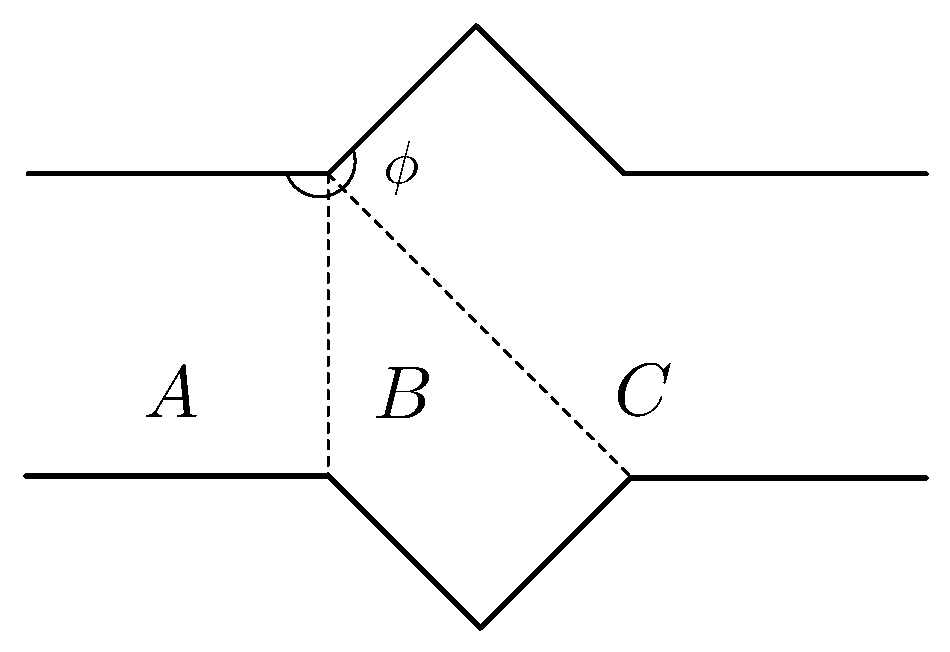
\includegraphics[scale=0.45]{Figures/WallCase.pdf} 
\caption{}\label{fig:wallcase}
\end{figure}

\subsection{The force at doorways}
We encountered a problem when dealing with doors. The problem arises because 
the door is constructed by two free endpoints and pedestrians feel a repulsion 
force from these points according to section \ref{wallEndpoints}. This means 
that a pedestrians trying to exit through the door will feel a repulsive force 
from the walls which prevent him from walking through the door. The second he 
passes through the door he will be pushed forward and accelerate which is unwanted 
behaviour. This we resolved by removing the force from free endpoint when:

\begin{equation}
\| y - w \| > R
\end{equation}

This creates what we could call a "non repulsion zone" see figure(Mikkel Lav Tegning!).
In rare cases it could happen that a pedestrian is trying to exit the room and he feels 
no repulsion because he is in the "non repulsive zone", he is then pushed sideways out 
of the "non repulsion zone" and suddenly he will feel a great repulsive force because 
he first "discovers" it when he is very close to the wall see figure(Mikkel Lav Tegning!).
